\chapter{Design}
\label{ch:design}
In this section the theoretical foundations are used to design a viable
solution, accordingly to the requirements and constraints listed.
In the design phase, the product development starts, specifying the system in
terms of hardware and software and its associated interfaces, the error handling
required, and the design verification.
%
  \vspace{-5mm}
%  
\section{Hardware specification}
\label{sec:hw-specs}
The first step for system design is the \gls{hw} specification. This can be
pictured as a block diagram, ideally with \gls{cots}
components. Fig.~\ref{fig:block-diag} depicts the overall information flow and
the TV remote block diagram: the \texttt{User} interacts with
the TV remote by pressing buttons which triggers the emission of \gls{ir} codes
to the TV, containing the \gls{ir} receiver. As supported by the market research
seen in
Section~\ref{sec:market-research}, the block diagram of the TV remote control
can be taught of a physical input interface --- the pushbuttons, a processing
interface --- a microprocessor --- to determine which keys are pressed and the
resulting \gls{ir} codes to be emitted, and a \gls{ir} transmitter circuit as
the output where the IR LED also works as a visual output. Usually, there will
be also a digital interface, to handle the large amount of keys as a
\gls{io} expander with serial interface, e.g. the Microchip MCP23008/MCP23S08~\cite{microchip}, which is considered here for future expansibility of the device,
thus making it scalable. This can be especially useful when using
microprocessor units with lower I/O inputs. A tradeoff between the inclusion of
the multiplexer versus future redesign must be performed.

The microprocessor chosen depends on various factors, such as: architecture,
throughput, memory, processing power, power efficiency, toolchain availability
and programming easiness, etc. Additionally, one may consider the usage of a
microcontroller, due to added peripherals, easing the \gls{sw} burden. For
example, the usage of the \gls{pca} peripheral in the 8051 \gls{mcu} can free the processor from the
job of bit-banging the IR transmitter circuitry or the \gls{i2c} or \gls{spi} peripherals to
interface the I/O expander. With that said, the choice
relied on the 8051 MCU due to its small footprint, clock speed of up to 48 MHz,
low power usage on idle, the acquaintance with the toolchain and the
programming, and for the inclusion of the PCA, SPI and I2C peripherals.  
%
  \vspace{-5mm}
%  
%- Block diagram with COTS components, if possible
%- List of constraints of functions to be implemented in HW or SW
%  - Inclusion of a multiplexer may reduce SW burden
%  - CPU peripherals:
%  - PCA for wave generation
%  
\begin{figure}[htb!]
\centering
    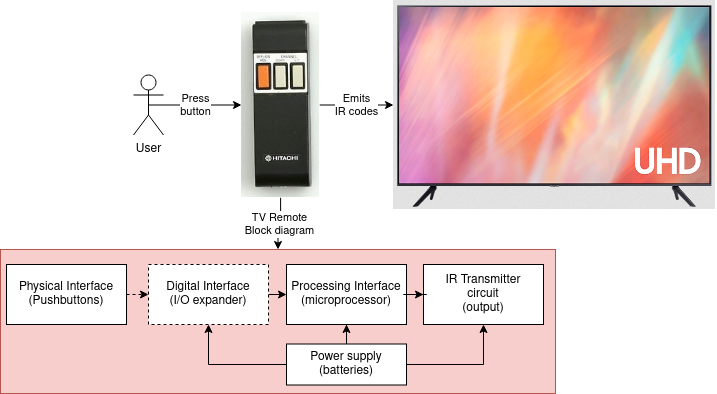
\includegraphics[width=0.7\columnwidth]{./img/block-diagram.png}
  \caption{Overall information flow and TV remote block diagram}%
\label{fig:block-diag}
\end{figure}
%
  \vspace{-5mm}
%  
\section{Hardware interfaces definition}
\label{sec:hw-interf-def}
After specifying the \gls{hw}, it is important to define its interfaces. The
TV remote control is clearly an event-driven asynchronous system, thus using HW
interrupts. When a user presses a pushbutton that event should be signaled to
the \gls{cpu} of the MCU via an external interrupt, ``waking'' it up. The CPU
handles that interrupt via an \gls{isr}, processing it and actuating, if
required. The system then goes back to sleep.

The 8051 MCU only contains 2 external interrupts sources --- \texttt{EXT0} and
\texttt{EXT1} --- thus limitting the direct connection of the pushbuttons to the
MCU, even with the pull-up circuitry. This is where the serial I/O expander
becomes most useful, as it can be connected to TV remote keys (up to 8 in this
case) and connected to a single external interrupt pin, being then read via
\gls{i2c} or \gls{spi} interface. Thus, the keys can be connected through
pull-up circuitry to the I/O expander and the output is then connected to
\texttt{EXT0} on the 8051 MCU. The communication protocol chosen is \gls{i2c} as
it is more expandable

Concerning the output, the 8051 PCA peripheral is connected to the IR
transmitter circuitry, for IR code emission.
%
  \vspace{-5mm}
%  
\section{Software specification}
\label{sec:sw-specs}
Top-down methodology
1. Identify main subsystems
   1. Signal input detector
   2. Event handler
   3. Output generator
%
  \vspace{-5mm}
%  
\section{Software interfaces definition}
\label{sec:sw-interf-def}
- Define the APIs in detail:
  - header files with:
    - functions prototypes
    - data structure declarations
    - class declarations

\section{Start-up/shutdown process specification}
\label{sec:startup-shutdown}
%
  \vspace{-5mm}
%  
\section{Error handling specification}
\label{sec:error-handling-specification}
- Create error-handling routines
- Watchdog timer can be used for system recovery
%
  \vspace{-5mm}
%  
\section{Design verification}
\label{sec:design-verification}
%
  \vspace{-5mm}
%  
%%% Local Variables:
%%% mode: latex
%%% TeX-master: "../../dissertation"
%%% End:
